\begin{definition}\label{conj_elem}  Un conjunto  $D\subseteq\Rn{2}$ se llama elemental si  puede ser descripto de alguna de las siguientes maneras. 
   
    \begin{enumerate}
    \item[i.] Si  existen funciones $\phi_1,\;\phi_2:[a,b]\to\R$  continuas  tales que $ \phi_1(x) < \phi_2(x) \: \forall x \in (a,b) $  y:
    \begin{equation}\label{def:tipo1}
     D = \{ (x,y) \in \mathbb{R}^{2}: \:   x\in[a,b] \: \land \: \phi_1(x)\leq y\leq\phi_2(x) ;\forall\;x\in[a,b] \}  
     \end{equation}   En tal caso  el conjunto $D$ se llama  \textit{elemental de tipo 1.} 
   
    \item[ii.]Si existen funciones $\psi_1,\;\psi_2:[c,d]\to\R$  continuas tales que $ \psi_1(y) < \psi_2(y) \: \forall y \in (c,d)$ y 
    \begin{equation}\label{def:tipo2}
     D = \{ (x,y) \in \mathbb{R}^{2}:   y\in[c,d] \: \land \:  \psi_1(y)\leq x\leq\psi_2(y) ;\forall\;y\in[c,d] \}  
     \end{equation}
     En tal caso el conjunto $D$  se llama  \textit{elemental de tipo 2.} 
    
    \item[iii.] $D$ se llama conjunto elemental de \textit{tipo 3} si es \textit{tipo 1} y \textit{tipo 2} a la vez.
    
    \input{figs/conj-elementales.tex}
    
    \end{enumerate}
\end{definition}

\begin{example}
    Para poder clasificar a una regi\'on como tipo 3 es necesario poder encontrar simult\'aneamente funciones $\phi_1$, $\phi_2$, $\psi_1$ y $\psi_2$ tales que
    \[
    \begin{dcases}
        \phi_1(x)\leq y\leq\phi_2(x) & x\in[a,b]\\[.2cm]
        \psi_1(y)\leq x\leq\psi_2(y) & y\in[c,d].
    \end{dcases}
    \]
    Un ejemplo simple de tal regi\'on es un c\'irculo, donde la ecuaci\'on de esta regi\'on es $$D=\{(x,y)\in\Rn{2}:(x-x_0)^2+(y-y_0)^2\leq r\}.$$  

    \input{figs/ex_tipo3.tex}

    Para describir esta regi\'on como Tipo $1$  debemos despejar $y$ en funci\'on de $x$, esto es,
 
 \textcolor{red}{Agregar los dos dibujos marcando claramete cada una de las situaciones }

   \[
        \phi_1(x)=-\sqrt{r-(x-x_0)^2}+y_0,\quad x\in[x_0-r,x_0+r],
    \]
    y
    \[
        \phi_2(x)=\sqrt{r-(x-x_0)^2}+y_0,\quad x\in[x_0-r,x_0+r].
    \]

    Puede observarse que $D$ es una regi\'on de tipo 1:

    \begin{center}
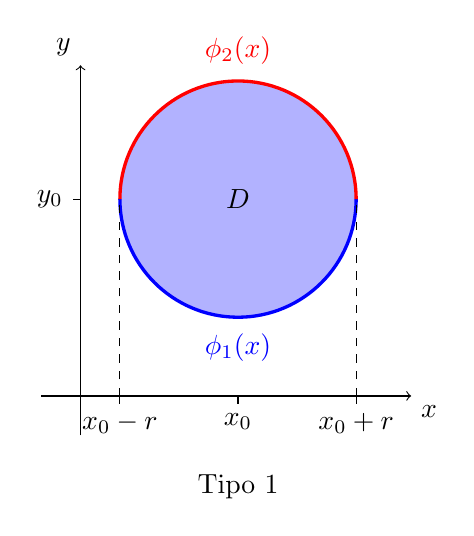
\begin{tikzpicture}
    % parámetros
    \def\cx{2}    % x_0
    \def\cy{2.5}    % y_0
    \def\rr{1.5}  % r

    %—————— Región Tipo 1 (despeje de y en función de x) ——————
    \begin{scope}
        % ejes
        \draw[->] (-0.5,0) -- (4.2,0) node[below right] {$x$};
        \draw[->] (0,-0.5) -- (0,4.2) node[above left]  {$y$};

        % relleno del círculo
        \fill[blue!30] (\cx,\cy) circle [radius=\rr];

        % semicircunferencia inferior: phi_1(x) = -sqrt(r-(x-x0)^2)+y0
        \draw[blue, very thick] (\cx-\rr,\cy) arc[start angle=180, end angle=360, radius=\rr]
            node[midway, below, yshift=-2pt] {\color{blue}$\phi_1(x)$};
        % semicircunferencia superior: phi_2(x) = +sqrt(r-(x-x0)^2)+y0
        \draw[red, very thick] (\cx-\rr,\cy) arc[start angle=180, end angle=0, radius=\rr]
            node[midway, above, yshift=2pt] {\color{red}$\phi_2(x)$};

        % líneas punteadas verticales en x_0 - r y x_0 + r
        \draw[dashed] (\cx-\rr,0) -- (\cx-\rr,\cy);
        \draw[dashed] (\cx+\rr,0) -- (\cx+\rr,\cy);

        % ticks y etiquetas en el eje x
        \draw (\cx-\rr,0) -- ++(0,-0.1) node[below] {$x_0-r$};
        \draw (\cx,0)     -- ++(0,-0.1) node[below] {$x_0$};
        \draw (\cx+\rr,0) -- ++(0,-0.1) node[below] {$x_0+r$};
        % tick y etiqueta en y_0
        \draw (0,\cy) -- ++(-0.1,0) node[left] {$y_0$};

        % etiqueta D
        \node at (\cx,\cy) {$D$};

        % título
        \node[below, yshift=-22pt] at (\cx,-0.1) {Tipo 1};
    \end{scope}
    \end{tikzpicture}
    \end{center}


    A su vez,  para describir esta regi\'on como Tipo $2$  debemos despejar $x$ en funci\'on de $y$, esto es, 
    \[
        \psi_1(y)=-\sqrt{r-(y-y_0)^2}+x_0,\quad y\in[y_0-r,y_0+r],
    \]
    y
    \[
        \psi_2(y)=\sqrt{r-(y-y_0)^2}+x_0,\quad y\in[y_0-r,y_0+r].
    \]
    Puede observarse que $D$ es una regi\'on de tipo 2:
    \begin{center}
        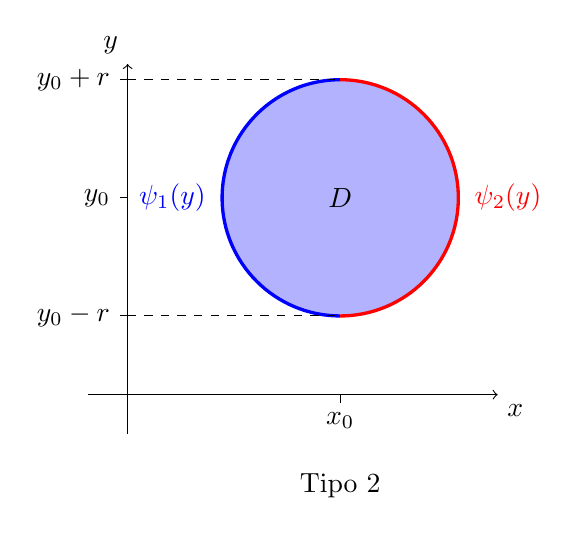
\begin{tikzpicture}
     \begin{scope}[xshift=7cm]
        \def\cxx{2.7}
        \def\cx{2}    % x_0
        \def\cy{2.5}    % y_0
        \def\rr{1.5}  % r

        % ejes
        \draw[->] (-0.5,0) -- (4.7,0) node[below right] {$x$};
        \draw[->] (0,-0.5) -- (0,4.2) node[above left]  {$y$};

        % relleno del círculo
        \fill[blue!30] (\cxx,\cy) circle [radius=\rr];

        % semicircunferencia izquierda: psi_1(y) = -sqrt(r-(y-y0)^2)+x0
        \draw[blue, very thick] (\cxx,\cy-\rr) arc[start angle=270, end angle=90, radius=\rr]
            node[midway, left, xshift=-2pt] {\color{blue}$\psi_1(y)$};
        % semicircunferencia derecha: psi_2(y) = +sqrt(r-(y-y0)^2)+x0
        \draw[red, very thick] (\cxx,\cy-\rr) arc[start angle=-90, end angle=90, radius=\rr]
            node[midway, right, xshift=2pt] {\color{red}$\psi_2(y)$};

        % líneas punteadas horizontales en y_0 - r y y_0 + r
        \draw[dashed] (0,\cy-\rr) -- (\cxx,\cy-\rr);
        \draw[dashed] (0,\cy+\rr) -- (\cxx,\cy+\rr);

        % ticks y etiquetas en el eje y
        \draw (0,\cy-\rr) -- ++(-0.1,0) node[left] {$y_0-r$};
        \draw (0,\cy)     -- ++(-0.1,0) node[left] {$y_0$};
        \draw (0,\cy+\rr) -- ++(-0.1,0) node[left] {$y_0+r$};
        % tick y etiqueta en x_0
        \draw (\cxx,0) -- ++(0,-0.1) node[below] {$x_0$};

        % etiqueta D
        \node at (\cxx,\cy) {$D$};

        % título
        \node[below, yshift=-22pt] at (\cxx,-0.1) {Tipo 2};
    \end{scope}
\end{tikzpicture}
\end{center}
    Por tanto, $D$ es una regi\'on de tipo 3.
\end{example}

